\section{可解析的模型}
\label{sec:rd-analytic}

编码定理把问题交还给式~\eqref{eq:rd-information-rd}的优化。少数模型可以精确求解，办法都是两步：先证明一个对所有满足失真约束的测试信道都成立的互信息下界，再构造一个测试信道使下界取等号。下界说“不可能更省”，构造说“确实能做到”，两者相遇处就是$R(D)$。

构造时常常反过来想：不直接写$q(\hat{x}\mid x)$，而是先给出$\hat{X}$的分布，再说明$X$怎样由$\hat{X}$加上一个独立的“误差”得到。这种从重构到源的描述称为\term{反向测试信道}（backward test channel）。只要它产生的$X$恰好服从给定的源分布，对$X$取条件就得到一个普通的测试信道。

\subsection{二元信源}
\label{sec:rd-binary}

开头的雨天记录现在可以算到底。设$X\sim\operatorname{Bern}(p)$，失真为Hamming失真。交换符号$0$与$1$不改变问题，所以不妨设$p\leq\tfrac12$。由第~\ref{sec:rd-feasible-range}节，$D_{\min}=0$，$D_{\max}=p$，零码率时一律输出更常见的$0$。

\begin{theorem}[二元信源的率失真函数]
\label{thm:rd-binary}
设$X\sim\operatorname{Bern}(p)$，$0\leq p\leq\tfrac12$，失真为式~\eqref{eq:rd-hamming}。则
\begin{equation}
  R(D)=\begin{cases}
    h_2(p)-h_2(D), & 0\leq D\leq p,\\
    0, & D\geq p.
  \end{cases}
  \label{eq:rd-binary}
\end{equation}
\end{theorem}

\begin{proof}
$D\geq p$时由定理~\ref{thm:rd-zero-rate}得$R(D)=0$。下面设$0\leq D<p$，于是$p>0$。

\emph{下界。}任取满足$\mathbb{E}d\leq D$的测试信道，令$E=X\oplus\hat{X}$为模$2$和，$E=1$表示重构出错，$\mathbb{P}(E=1)=\mathbb{E}d\leq D$。给定$\hat{X}$时，$X\mapsto X\oplus\hat{X}$是一一对应，条件熵不变，所以
\[
  H(X\mid\hat{X})=H(E\mid\hat{X})\leq H(E)=h_2\bigl(\mathbb{P}(E=1)\bigr)\leq h_2(D).
\]
最后一步用了$h_2$在$[0,\tfrac12]$上递增，以及$\mathbb{P}(E=1)\leq D<\tfrac12$。于是
\[
  I(X;\hat{X})=H(X)-H(X\mid\hat{X})\geq h_2(p)-h_2(D).
\]

\emph{达到下界。}令
\[
  r=\frac{p-D}{1-2D}.
\]
由$0\leq D<p\leq\tfrac12$，分子与分母都为正；又$p\leq\tfrac12<1-D$，所以$p-D<1-2D$，$r\in(0,1)$。取相互独立的$\hat{X}\sim\operatorname{Bern}(r)$与$Z\sim\operatorname{Bern}(D)$，令$X=\hat{X}\oplus Z$。

$X=1$当且仅当$\hat{X}$与$Z$恰有一个为$1$，
\[
  \mathbb{P}(X=1)=r(1-D)+(1-r)D=D+r(1-2D)=p ,
\]
所以$X$恰好服从源分布，$(X,\hat{X})$的联合分布给出一个测试信道。它的失真是$\mathbb{P}(X\neq\hat{X})=\mathbb{P}(Z=1)=D$。$Z$与$\hat{X}$独立，
\[
  I(X;\hat{X})=H(X)-H(X\mid\hat{X})=h_2(p)-H(Z\mid\hat{X})=h_2(p)-h_2(D),
\]
与下界相等。
\end{proof}

下界的证明说明了等号何时成立：错误指示$E$必须与$\hat{X}$独立，并且错误率恰为$D$。构造的反向测试信道正好满足这两点。图~\ref{fig:rd-binary-test-channels}(a)画出$p=0.3$、$D=0.1$时的反向信道：$\hat{X}\sim\operatorname{Bern}(0.25)$，再以$0.1$的概率翻转，得到$\operatorname{Bern}(0.3)$。

用Bayes公式换回从$X$到$\hat{X}$的方向。$X=0$而$\hat{X}=1$需要$\hat{X}=1$且$Z=1$；$X=1$而$\hat{X}=0$需要$\hat{X}=0$且$Z=1$。于是
\[
  \begin{aligned}
  q(1\mid0)&=\frac{rD}{1-p}=\frac{0.25\times0.1}{0.7}=\frac1{28},\\
  q(0\mid1)&=\frac{(1-r)D}{p}=\frac{0.75\times0.1}{0.3}=\frac14 ,
  \end{aligned}
\]
这就是第~\ref{sec:rd-test-channels}节第三个测试信道，图~\ref{fig:rd-binary-test-channels}(b)画出了它。由式~\eqref{eq:rd-binary}，
\[
  R(0.1)=h_2(0.3)-h_2(0.1)\approx0.8813-0.4690=0.4123 .
\]

\begin{BookInlineFigure}
  \centering
  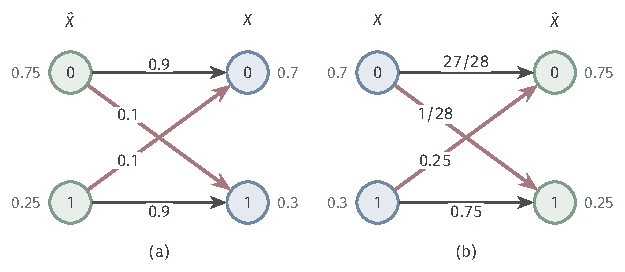
\includegraphics[width=106mm]{figures/07-probability/05-source-coding/tikz/rd-binary-test-channels/figure.pdf}
  \caption{$X\sim\operatorname{Bern}(0.3)$、Hamming失真、$D=0.1$的最优测试信道。(a)反向形式：绿色的$\hat{X}\sim\operatorname{Bern}(0.25)$经过独立的翻转（红箭头，概率$0.1$）得到蓝色的$X$，节点旁的数是边缘概率。(b)由Bayes公式得到的正向形式$q(\hat{x}\mid x)$，罕见符号$1$被改错的概率$\tfrac14$远大于常见符号$0$的$\tfrac1{28}$。}
  \label{fig:rd-binary-test-channels}
\end{BookInlineFigure}

开头的问题有了答案：允许错$10\%$，每天只需约$0.412$\,bit，不到无损所需$0.881$\,bit的一半，远少于按比例打折的$0.881\times0.9\approx0.793$。第~\ref{sec:rd-block-model}节中要求每一块都不超过$10\%$错误时至少需要$0.531$\,bit；期望失真要求允许少数块错得多，于是更省。

\paragraph{源概率与端点}
图~\ref{fig:rd-binary-curves}画出三个源概率下的曲线，可以对照式~\eqref{eq:rd-binary}逐项检查。
\begin{itemize}
  \item $D=0$时$R(0)=h_2(p)=H(X)$，回到无损编码的熵。
  \item 曲线在$D_{\max}=p$处降到零，零码率失真由源概率决定：$p=0.1$时一律猜$0$只错$10\%$，$p=\tfrac12$时要错一半。
  \item 均匀信源$p=\tfrac12$时$R(D)=1-h_2(D)$，这只是$p$的一个取值，曲线最高，因为每个符号最难预测。
  \item 退化情形$p=0$时信源是常数$0$，$D_{\max}=0$，$R\equiv0$；这时$h_2(p)-h_2(D)$在$D>0$时为负，公式只能在$0\leq D\leq p$上使用。
\end{itemize}

曲线的斜率是$R'(D)=-h_2'(D)=-\log_2\frac{1-D}{D}$，$D\downarrow0$时趋于$-\infty$。允许极少量的错误就能省下相当多的码率，这是有损压缩在低失真端最划算的原因；越往后，每多容忍一点失真省下的码率越少。

\begin{BookInlineFigure}
  \centering
  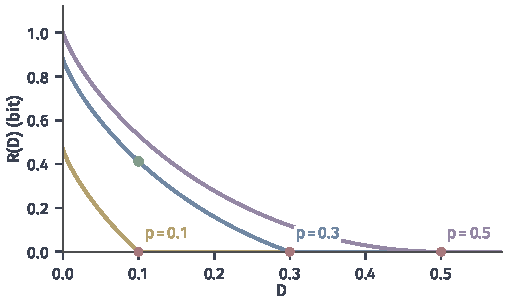
\includegraphics[width=86mm]{figures/07-probability/05-source-coding/matplotlib/rd-binary-curves/figure.pdf}
  \caption{$\operatorname{Bern}(p)$信源在Hamming失真下的$R(D)$，$p=0.1$（黄）、$0.3$（蓝）、$0.5$（紫）。红点是零码率失真$D_{\max}=p$，曲线在纵轴上的截距是$h_2(p)$。绿点是贯穿例子$(0.1,0.4123)$。}
  \label{fig:rd-binary-curves}
\end{BookInlineFigure}

\subsection{高斯信源}
\label{sec:rd-gaussian}

开头的第二个问题涉及实值信源与平方失真。这里重构值连续变化，第~\ref{sec:rd-coding-theorem}节的有限字母表证明不能直接搬用；我们先在信息率失真函数的层面上求解，再说明编码定理在这里的地位。计算需要一个关于微分熵的不等式，它也会在第~\ref{chap:gaussian-channel-capacity}章计算高斯信道容量时用到。

本小节沿用第~\ref{chap:information-measures}章的微分熵，换成以bit计：对有密度$f$的实值随机变量，
\[
  h(X)=-\int_{\mathbb{R}}f(x)\log_2f(x)\,\mathrm{d}x ,
\]
前提是这个积分有意义。KL散度同样以bit计，即在第~\ref{chap:distribution-comparison}章的定义中把$\ln$换成$\log_2$，它仍然非负，且为零当且仅当两个分布相同。

\subsubsection{高斯分布的熵上界}
\label{sec:rd-gaussian-entropy}

方差固定时，哪种分布的不确定性最大？图~\ref{fig:rd-gaussian-entropy}中三个密度均值都是$0$、方差都是$1$。均匀分布把质量平铺在$[-\sqrt3,\sqrt3]$上，Laplace分布尖峰更高、尾部更厚，高斯分布介于两者之间。它们的微分熵分别是
\[
  \log_2(2\sqrt3)\approx1.792,\qquad \log_2(\sqrt2\,\mathrm{e})\approx1.943,\qquad \frac12\log_2(2\pi\mathrm{e})\approx2.047 ,
\]
第二个用了Laplace分布$\operatorname{Laplace}(0,b)$的方差$2b^{2}=1$与熵$\log_2(2\mathrm{e}b)$。高斯最大，这不是巧合。

\begin{BookInlineFigure}
  \centering
  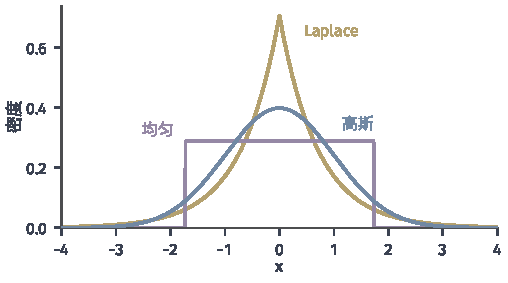
\includegraphics[width=86mm]{figures/07-probability/05-source-coding/matplotlib/rd-gaussian-entropy/figure.pdf}
  \caption{均值为$0$、方差为$1$的三个密度：标准高斯（蓝，$h\approx2.047$\,bit）、$\operatorname{Laplace}(0,1/\sqrt2)$（黄，$h\approx1.943$\,bit）、$[-\sqrt3,\sqrt3]$上的均匀分布（紫，$h\approx1.792$\,bit）。三个熵值也用数值积分核对过。}
  \label{fig:rd-gaussian-entropy}
\end{BookInlineFigure}

\begin{theorem}[固定方差的熵上界]
\label{thm:rd-gaussian-max-entropy}
设实值随机变量$X$有密度$f$，均值为$\mu$，方差$\sigma^{2}\in(0,\infty)$。则定义$h(X)$的积分有意义，取值于$[-\infty,\infty)$，并且
\begin{equation}
  h(X)\leq\frac12\log_2(2\pi\mathrm{e}\sigma^{2}),
  \label{eq:rd-gaussian-max-entropy}
\end{equation}
等号成立当且仅当$X\sim\mathcal{N}(\mu,\sigma^{2})$。
\end{theorem}

\begin{proof}
取同均值、同方差的高斯密度作参考，
\[
  g(x)=\frac{1}{\sqrt{2\pi\sigma^{2}}}\exp\Bigl(-\frac{(x-\mu)^{2}}{2\sigma^{2}}\Bigr).
\]
先算$-\log_2g$在$f$下的期望。由$g$的表达式，
\[
  -\log_2g(x)=\frac12\log_2(2\pi\sigma^{2})+(\log_2\mathrm{e})\frac{(x-\mu)^{2}}{2\sigma^{2}},
\]
它是$x$的二次函数，在$f$下可积。由$\mathbb{E}(X-\mu)^{2}=\sigma^{2}$，
\[
  -\int f\log_2g\,\mathrm{d}x=\frac12\log_2(2\pi\sigma^{2})+\frac{\log_2\mathrm{e}}{2}=\frac12\log_2(2\pi\mathrm{e}\sigma^{2}).
\]

再看KL散度的被积函数$f\log_2(f/g)$（在$f>0$处）。由$\ln t\geq1-1/t$，
\[
  f\ln\frac{f}{g}\geq f-g ,
\]
所以它的负部不超过$g$，可积。于是KL散度
\[
  D_{\mathrm{KL}}(f\Vert g)=\int f\log_2\frac{f}{g}\,\mathrm{d}x
\]
有意义，取值于$[0,\infty]$。

在$f>0$处写$f\log_2f=f\log_2(f/g)+f\log_2g$。右端第一项负部可积，第二项可积，所以$f\log_2f$的负部可积，$\int f\log_2f\,\mathrm{d}x$有意义且大于$-\infty$。这说明$h(X)$有意义，取值于$[-\infty,\infty)$，并且
\[
  h(X)=-\int f\log_2\frac{f}{g}\,\mathrm{d}x-\int f\log_2g\,\mathrm{d}x=\frac12\log_2(2\pi\mathrm{e}\sigma^{2})-D_{\mathrm{KL}}(f\Vert g).
\]
KL散度非负，得到式~\eqref{eq:rd-gaussian-max-entropy}。等号成立当且仅当$D_{\mathrm{KL}}(f\Vert g)=0$，即$f=g$几乎处处，也就是$X\sim\mathcal{N}(\mu,\sigma^{2})$。
\end{proof}

证明里的关键是：$-\log_2g$只是$x$的二次函数，它在任何同方差分布下的平均都一样。于是“$f$的熵比高斯少多少”恰好就是$f$与高斯的KL散度。条件中的方差有限保证了这个平均有限；$h(X)$可以是$-\infty$（例如密度在某些点附近极度集中），不等式仍然成立，只是没有信息量。没有方差限制时，微分熵没有上界：$\operatorname{Unif}(0,a)$的熵$\log_2a$随$a$无限增大。

\subsubsection{高斯率失真函数}
\label{sec:rd-gaussian-rd}

设$X\sim\mathcal{N}(\mu,\sigma^{2})$，$\sigma^{2}>0$，失真为平方误差。测试信道是从$\mathbb{R}$到$\mathbb{R}$的Markov核，$R(D)$仍按式~\eqref{eq:rd-information-rd}定义，互信息是联合分布相对边缘乘积的KL散度，可以为$+\infty$。

\begin{theorem}[高斯信源的率失真函数]
\label{thm:rd-gaussian}
在上述设定下，
\begin{equation}
  R(D)=\begin{cases}
    \dfrac12\log_2\dfrac{\sigma^{2}}{D}, & 0<D<\sigma^{2},\\
    0, & D\geq\sigma^{2},
  \end{cases}
  \label{eq:rd-gaussian}
\end{equation}
且$R(0)=+\infty$。单位是bit每个实值源符号。
\end{theorem}

\begin{proof}
把$X$与$\hat{X}$同时减去$\mu$，平方误差与互信息都不变，所以不妨设$\mu=0$。$D\geq\sigma^{2}$时恒输出$0$，失真为$\mathbb{E}X^{2}=\sigma^{2}\leq D$，互信息为零。下面设$0<D<\sigma^{2}$，分下界与达到两部分。

\emph{下界的分解。}任取满足$\mathbb{E}(X-\hat{X})^{2}\leq D$的联合分布。若$I(X;\hat{X})=+\infty$无需证明，下设它有限。这时联合分布对$P_X\otimes P_{\hat{X}}$绝对连续，记Radon–Nikodym导数为$\lambda(x,\hat{x})$，则互信息是$\log_2\lambda(X,\hat{X})$的期望。$P_X$有密度$f=\varphi_{\sigma^{2}}$（方差为$\sigma^{2}$的零均值高斯密度），所以给定$\hat{X}=\hat{x}$时$X$的条件分布有密度$p(x\mid\hat{x})=\lambda(x,\hat{x})f(x)$，并且
\[
  I(X;\hat{X})=\mathbb{E}\Bigl[\log_2\frac{p(X\mid\hat{X})}{f(X)}\Bigr].
\]

\emph{条件高斯参考。}引入一个“猜测”的条件密度$w(x\mid\hat{x})=\varphi_D(x-\hat{x})$，即以$\hat{x}$为中心、方差为$D$的高斯密度。把对数拆成两项：
\[
  \log_2\frac{p(X\mid\hat{X})}{f(X)}=\log_2\frac{p(X\mid\hat{X})}{w(X\mid\hat{X})}+\log_2\frac{w(X\mid\hat{X})}{f(X)} .
\]
第二项写开是
\[
  \frac12\log_2\frac{\sigma^{2}}{D}-\frac{\log_2\mathrm{e}}{2}\Bigl(\frac{(X-\hat{X})^{2}}{D}-\frac{X^{2}}{\sigma^{2}}\Bigr),
\]
由$\mathbb{E}X^{2}=\sigma^{2}$与$\mathbb{E}(X-\hat{X})^{2}\leq D$，它可积，期望至少为
\[
  \frac12\log_2\frac{\sigma^{2}}{D}-\frac{\log_2\mathrm{e}}{2}\,(1-1)=\frac12\log_2\frac{\sigma^{2}}{D}.
\]

\emph{条件KL非负。}左端与第二项都可积，所以第一项可积。对$\hat{X}$取条件，第一项的条件期望是条件分布$p(\cdot\mid\hat{X})$相对参考$w(\cdot\mid\hat{X})$的KL散度，非负；再对$\hat{X}$平均仍非负。于是
\[
  I(X;\hat{X})\geq\frac12\log_2\frac{\sigma^{2}}{D}.
\]

\emph{达到下界。}取相互独立的$\hat{X}\sim\mathcal{N}(0,\sigma^{2}-D)$与$Z\sim\mathcal{N}(0,D)$，令$X=\hat{X}+Z$。独立高斯之和仍是高斯，$X\sim\mathcal{N}(0,\sigma^{2})$，失真$\mathbb{E}(X-\hat{X})^{2}=\mathbb{E}Z^{2}=D$。这时条件密度$p(\cdot\mid\hat{x})$恰是参考$w(\cdot\mid\hat{x})$，第一项恒为零；第二项中$\mathbb{E}(X-\hat{X})^{2}=D$，期望恰为$\tfrac12\log_2(\sigma^{2}/D)$。下界取到。

\emph{零失真。}$D=0$时可行的联合分布必须满足$\hat{X}=X$几乎必然，联合分布集中在对角线上，而$P_X\otimes P_X$给对角线的概率为零，联合分布不对乘积绝对连续，互信息为$+\infty$。
\end{proof}

\paragraph{改写成熵差}
当相关的微分熵都有限时，上面的下界有一个更直观的读法。此时$I(X;\hat{X})=h(X)-h(X\mid\hat{X})$。给定$\hat{X}$后，$X$与误差$X-\hat{X}$只差一个已知的平移，条件熵相同；条件化不增加熵；再对误差用定理~\ref{thm:rd-gaussian-max-entropy}，其方差不超过$\mathbb{E}(X-\hat{X})^{2}\leq D$：
\[
  h(X\mid\hat{X})=h(X-\hat{X}\mid\hat{X})\leq h(X-\hat{X})\leq\frac12\log_2(2\pi\mathrm{e}D).
\]
于是
\[
  I(X;\hat{X})\geq\frac12\log_2(2\pi\mathrm{e}\sigma^{2})-\frac12\log_2(2\pi\mathrm{e}D)=\frac12\log_2\frac{\sigma^{2}}{D},
\]
与定理一致：重构后剩下的不确定性，至多是一个方差为$D$的高斯误差的不确定性。

这个读法要求每个熵项都有意义且有限，否则会出现“无穷减无穷”；例如$\hat{X}$只取有限个值时，给定$\hat{X}$后$X$的条件熵要逐值核对。上面的证明只用条件KL，不需要这些前提，两者的数学内容相同：熵上界的证明本身就是相对高斯参考的KL非负。

\paragraph{几何图景}
达到下界的反向测试信道是$X=\hat{X}+Z$，$\hat{X}$与$Z$独立。在均方意义下，独立且零均值就是正交，于是$\sigma^{2}=(\sigma^{2}-D)+D$是一个勾股关系，图~\ref{fig:rd-gaussian-geometry}画出了这个直角三角形。最优重构是源的一个“缩短的影子”：它的方差只有$\sigma^{2}-D$，不是$\sigma^{2}$。

从$X$看，$(X,\hat{X})$是联合高斯，$\operatorname{Cov}(X,\hat{X})=\sigma^{2}-D$。记$a=1-D/\sigma^{2}$，由二元高斯的条件分布，
\[
  \mathbb{E}[\hat{X}\mid X]=aX,\qquad \operatorname{Var}(\hat{X}\mid X)=(\sigma^{2}-D)-\frac{(\sigma^{2}-D)^{2}}{\sigma^{2}}=aD .
\]
所以正向测试信道是$q(\cdot\mid x)=\mathcal{N}(ax,aD)$：先把$x$向$0$收缩到$ax$，再加上方差为$aD$的独立噪声。

\begin{BookInlineFigure}
  \centering
  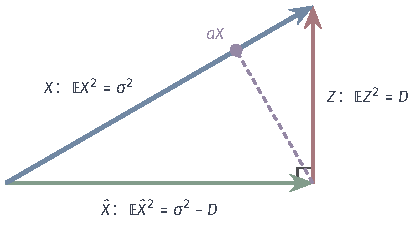
\includegraphics[width=72mm]{figures/07-probability/05-source-coding/tikz/rd-gaussian-geometry/figure.pdf}
  \caption{高斯最优测试信道的均方几何，$\sigma^{2}=1$，$D=\tfrac14$。向量长度表示均方根：绿色$\hat{X}$与红色误差$Z$独立因而正交，合成蓝色的$X$。紫点是$\hat{X}$在$X$方向上的投影$aX$，$a=1-D/\sigma^{2}=\tfrac34$，紫色虚线垂直于$X$。}
  \label{fig:rd-gaussian-geometry}
\end{BookInlineFigure}

\paragraph{各个区间的码率}
式~\eqref{eq:rd-gaussian}的三段各有含义。
\begin{itemize}
  \item $0<D<\sigma^{2}$时，反解得失真率函数$D(R)=\sigma^{2}2^{-2R}$：每多$1$\,bit，均方误差降为四分之一。$\sigma^{2}=1$、$D=\tfrac14$时恰需$1$\,bit。
  \item $D\geq\sigma^{2}$时不需要描述，输出均值即可，零码率失真就是方差。
  \item $D\downarrow0$时$R(D)\to\infty$：连续取值的信源不能用有限码率精确描述，这与有限字母表上$R(0)=H(X)$的情形不同。
\end{itemize}
均值$\mu$只影响平移，不改变码率。退化的$\sigma^{2}=0$是确定的源$X=\mu$，对一切$D\geq0$有$R(D)=0$，公式~\eqref{eq:rd-gaussian}不适用。

\paragraph{编码定理与有限量化器}
定理~\ref{thm:rd-gaussian}是关于信息率失真函数的结论。要说$R(D)$也是高斯信源在平方失真下的最低渐近码率，还需要把编码定理推广到连续字母表与无界失真：可以先把源与重构离散化、截断尾部，在有限字母表上用第~\ref{sec:rd-coding-theorem}节的定理，再控制离散化与尾部带来的误差。结论成立，但证明较长，读者可查阅~\scite{math-cover2006information}。

承认这一点，就能回答开头的第二个问题。图~\ref{fig:rd-gaussian-quantizers}对标准高斯信源比较几类方案。码率为$1$\,bit时，极限是$D(1)=0.25$，而第~\ref{chap:quantization}章的两点最优量化器只做到$1-2/\pi\approx0.363$。反过来看，失真$0.363$只需
\[
  R(0.363)=\frac12\log_2\frac{1}{0.363}\approx0.730
\]
bit，逐个量化多用了约$0.27$\,bit。四点、八点、十六点的Lloyd–Max量化器与极限之间也一直有差距。

\begin{BookInlineFigure}
  \centering
  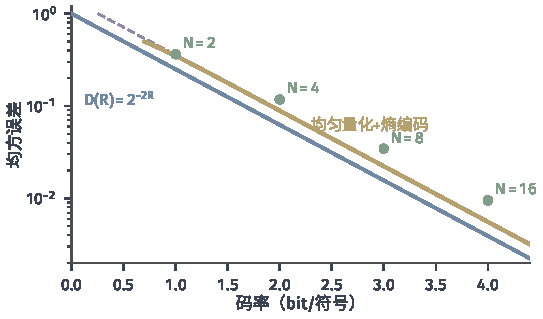
\includegraphics[width=92mm]{figures/07-probability/05-source-coding/matplotlib/rd-gaussian-quantizers/figure.pdf}
  \caption{标准高斯信源在平方失真下的码率与均方误差，纵轴为对数刻度。蓝线是$D(R)=2^{-2R}$。绿点是$N=2,4,8,16$个重构值的Lloyd–Max量化器，码率取定长索引的$\log_2N$。黄线是步长从$3$减小到$0.1$的均匀量化器（重构取区间条件均值），码率取索引的熵，即理想无损压缩索引后的平均长度。紫色虚线是蓝线向右平移$\tfrac12\log_2\frac{\pi\mathrm{e}}{6}\approx0.2546$\,bit。}
  \label{fig:rd-gaussian-quantizers}
\end{BookInlineFigure}

把均匀量化器的索引再作无损压缩（第~\ref{chap:quantization}章），黄线比定长索引好得多，但在高码率时与极限保持一个固定的水平距离。这个距离可以用高分辨率近似估计。步长$\Delta$很小时，均方误差约为$\Delta^{2}/12$，索引的熵约为$h(X)-\log_2\Delta$，所以码率约为
\[
  h(X)-\frac12\log_2(12D).
\]
而由式~\eqref{eq:rd-gaussian}与$h(X)=\frac12\log_2(2\pi\mathrm{e}\sigma^{2})$，$R(D)=h(X)-\frac12\log_2(2\pi\mathrm{e}D)$。两者相减，差距约为
\[
  \frac12\log_2\frac{2\pi\mathrm{e}}{12}=\frac12\log_2\frac{\pi\mathrm{e}}{6}\approx0.2546
\]
bit。这只是近似推导，数值计算印证了它：步长$0.25$时，索引熵为$4.051$\,bit，均方误差为$0.00518$，而这个失真下的$R(D)$约为$3.796$\,bit，差$0.2546$\,bit。逐值量化的格子是一维区间，要再缩小这段差距，只能把许多值合在一起量化，这正是长块编码所做的事。

\subsection{多分量的码率分配}
\label{sec:rd-allocation}

一个测量向量有几个独立的高斯分量，方差各不相同，总的平方误差预算为$D$。码率该怎样分给各分量？直觉是方差大的分量多给，但给多少、方差小的分量是否要给，需要计算。

\paragraph{独立分量的分解}
设$\bm{X}=(X_1,\dots,X_m)$的分量相互独立，$X_k\sim\mathcal{N}(0,\sigma_k^{2})$，$\sigma_k^{2}>0$。把整个向量看成一个源符号，失真取$\lVert\bm{x}-\hat{\bm{x}}\rVert_2^{2}$，$R(D)$表示每个向量所需的bit数。记$R_k(D_k)$为第$k$个分量按式~\eqref{eq:rd-gaussian}的率失真函数，其中$\sigma^{2}$换成$\sigma_k^{2}$。

\begin{theorem}[反注水]
\label{thm:rd-reverse-waterfilling}
在上述设定下，对$0<D<\sum_k\sigma_k^{2}$，
\begin{equation}
  R(D)=\sum_{k=1}^{m}\frac12\log_2\frac{\sigma_k^{2}}{D_k},\qquad D_k=\min\{\theta,\sigma_k^{2}\},
  \label{eq:rd-reverse-waterfilling}
\end{equation}
其中$\theta>0$由$\sum_k\min\{\theta,\sigma_k^{2}\}=D$唯一确定；$D\geq\sum_k\sigma_k^{2}$时$R(D)=0$。
\end{theorem}

\begin{proof}
\emph{下界。}任取满足失真约束的联合分布，设互信息有限。由第~\ref{chap:information-measures}章互信息的链式法则，
\[
  I(\bm{X};\hat{\bm{X}})=\sum_{k=1}^{m}I(X_k;\hat{\bm{X}}\mid X_1,\dots,X_{k-1}).
\]
记$\bm{X}_{<k}=(X_1,\dots,X_{k-1})$，再用链式法则，
\[
  I(X_k;\hat{\bm{X}},\bm{X}_{<k})=I(X_k;\bm{X}_{<k})+I(X_k;\hat{\bm{X}}\mid\bm{X}_{<k}).
\]
分量独立使右端第一项为零，所以第$k$项等于$I(X_k;\hat{\bm{X}},\bm{X}_{<k})$，它不小于$I(X_k;\hat{X}_k)$（数据处理：丢掉一部分观测不增加信息）。

记$D_k=\mathbb{E}(X_k-\hat{X}_k)^{2}$，则$\sum_kD_k\leq D$，并由定理~\ref{thm:rd-gaussian}，$I(X_k;\hat{X}_k)\geq R_k(D_k)$。于是
\[
  I(\bm{X};\hat{\bm{X}})\geq\min\Bigl\{\sum_kR_k(D_k):\ D_k\geq0,\ \sum_kD_k\leq D\Bigr\}.
\]

\emph{达到。}对任意分配$(D_k)$，各分量独立地使用定理~\ref{thm:rd-gaussian}中的最优测试信道（$D_k\geq\sigma_k^{2}$时输出$0$）。各对$(X_k,\hat{X}_k)$相互独立，互信息可加，等于$\sum_kR_k(D_k)$，失真之和为$\sum_kD_k$。所以$R(D)$等于上面这个分配问题的最小值。

\emph{求解分配。}$D_k>\sigma_k^{2}$只浪费预算，可设$0<D_k\leq\sigma_k^{2}$，目标是$\sum_k\frac12\log_2(\sigma_k^{2}/D_k)$，凸且可微，约束是线性的。由KKT条件（可参考\BookChapterRef{chap:constrained-optimality}{卷五第17章“约束问题的最优性”}），存在$\nu\geq0$与$\eta_k\geq0$使
\[
  -\frac{\log_2\mathrm{e}}{2D_k}+\nu+\eta_k=0,\qquad \eta_k\,(D_k-\sigma_k^{2})=0 .
\]
若$D_k<\sigma_k^{2}$，则$\eta_k=0$，于是$\nu>0$，记
\[
  D_k=\frac{\log_2\mathrm{e}}{2\nu}=\theta .
\]
若$D_k=\sigma_k^{2}$，则
\[
  \frac{\log_2\mathrm{e}}{2\sigma_k^{2}}=\nu+\eta_k\geq\nu,
\]
即$\sigma_k^{2}\leq\theta$。两种情形合起来就是$D_k=\min\{\theta,\sigma_k^{2}\}$。凸问题中KKT条件也是充分的，所以这确实是最小点。$\theta\mapsto\sum_k\min\{\theta,\sigma_k^{2}\}$连续、严格递增直到$\sum_k\sigma_k^{2}$，所以$\theta$唯一。
\end{proof}

这个分配称为\term{反注水}（reverse water-filling）。把每个分量的方差画成一根柱子，在高度$\theta$处画一条水平线：高于水平线的分量，失真都是$\theta$，码率是$\frac12\log_2(\sigma_k^{2}/\theta)$；低于水平线的分量干脆不描述，输出$0$，失真就是它的全部方差。方差小的分量本身离$0$不远，花码率描述它不如把预算让给方差大的分量。

\paragraph{一个三分量的例子}
取$\sigma^{2}=(4,1,0.25)$，总失真$D=1.5$。试$\theta\in[0.25,1)$：第三个分量不描述，前两个失真都是$\theta$，
\[
  2\theta+0.25=1.5,\qquad \theta=0.625 ,
\]
确实落在所设区间内。各分量的码率为
\[
  R_1=\frac12\log_2\frac{4}{0.625}\approx1.339,\qquad
  R_2=\frac12\log_2\frac{1}{0.625}\approx0.339,\qquad R_3=0 .
\]
合计约$1.678$\,bit每向量，平均每个分量约$0.559$\,bit，平均每个分量的失真是$1.5/3=0.5$。总量与每分量平均量之间只差一个因子$m$，比较时两者不能混用。

作为对照，把预算平分，每个分量都给$0.5$。第三个分量的方差只有$0.25$，给它$0.5$的失真预算用不完，它实际只产生$0.25$的失真；前两个分量需要
\[
  \frac12\log_2\frac{4}{0.5}+\frac12\log_2\frac{1}{0.5}=1.5+0.5=2
\]
bit，比反注水多出约$0.32$\,bit，总失真却只有$1.25$，浪费了预算。

图~\ref{fig:rd-reverse-waterfilling}(a)画出这个分配，(b)画出总码率随总失真的变化。$D=0.75$时水平线降到$0.25$，第三个分量开始需要描述；$D=2.25$时水平线升到$1$，第二个分量不再描述。在这两个折点，曲线的组成方式改变，但仍连续且凸。

\begin{BookInlineFigure}
  \centering
  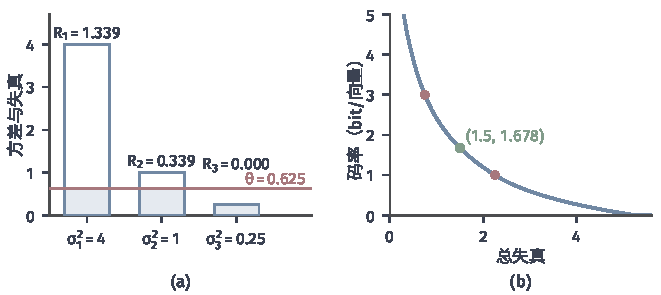
\includegraphics[width=112mm]{figures/07-probability/05-source-coding/matplotlib/rd-reverse-waterfilling/figure.pdf}
  \caption{方差为$(4,1,0.25)$的独立高斯分量的反注水。(a)总失真$1.5$时的分配：蓝框是各分量方差，浅蓝填充是分到的失真$D_k=\min\{\theta,\sigma_k^{2}\}$，红线是水平$\theta=0.625$，柱上方是各分量的码率（bit）。(b)每向量的总码率随总失真的变化；红点是分量开始或停止被描述的折点$D=0.75$与$D=2.25$，绿点是(a)中的分配。}
  \label{fig:rd-reverse-waterfilling}
\end{BookInlineFigure}

\paragraph{相关的高斯向量}
分量相关时先旋转坐标。设$\bm{X}\sim\mathcal{N}(\bm{0},\bm{\Sigma})$，协方差矩阵$\bm{\Sigma}$有正交特征分解$\bm{\Sigma}=\bm{U}\bm{\Lambda}\bm{U}^{\top}$，$\bm{\Lambda}$为特征值$\lambda_1,\dots,\lambda_m$组成的对角矩阵。令$\bm{Y}=\bm{U}^{\top}\bm{X}$，则$\bm{Y}\sim\mathcal{N}(\bm{0},\bm{\Lambda})$，各分量不相关。由第~\ref{chap:multivariate-distributions}章，联合高斯向量的分量不相关即独立。

旋转不改变问题。对任意重构$\hat{\bm{X}}$，令$\hat{\bm{Y}}=\bm{U}^{\top}\hat{\bm{X}}$。正交矩阵保持长度，
\[
  \lVert\bm{X}-\hat{\bm{X}}\rVert_2^{2}=\lVert\bm{Y}-\hat{\bm{Y}}\rVert_2^{2};
\]
$\bm{U}^{\top}$是可逆的连续映射，由第~\ref{chap:information-measures}章，双方向可测的一一变换保持互信息，$I(\bm{X};\hat{\bm{X}})=I(\bm{Y};\hat{\bm{Y}})$。所以两个问题的可行集合一一对应，目标值相同，$\bm{X}$的$R(D)$就是对特征值$\lambda_k$作反注水。

例如$\bm{\Sigma}=\begin{bmatrix}2&1\\1&2\end{bmatrix}$，特征值为$3$与$1$，特征向量为$(1,1)/\sqrt2$与$(-1,1)/\sqrt2$。总失真$D=1$时，试$\theta<1$，得$2\theta=1$，$\theta=0.5$，
\[
  R(1)=\frac12\log_2\frac{3}{0.5}+\frac12\log_2\frac{1}{0.5}\approx1.292+0.5=1.792
\]
bit每向量。若忽略相关性，把$X_1,X_2$当作两个方差为$2$的信源分别描述，最好的分法是各给$0.5$，需要$\frac12\log_2\frac{2}{0.5}\times2=2$\,bit。联合描述省下约$0.21$\,bit，来源于旋转后两个方向的方差不再相等，反注水可以把预算向方差大的方向倾斜。

\begin{BookInlineFigure}
  \centering
  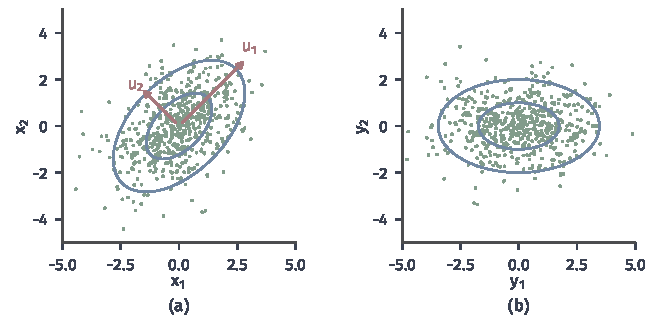
\includegraphics[width=112mm]{figures/07-probability/05-source-coding/matplotlib/rd-correlated-rotation/figure.pdf}
  \caption{相关高斯向量的旋转，$\bm{\Sigma}=\begin{bmatrix}2&1\\1&2\end{bmatrix}$，$600$个样本（绿），随机种子$722$。(a)原坐标中的样本与一倍、两倍标准差的等密度椭圆（蓝），红箭头是特征方向$\bm{u}_1,\bm{u}_2$。(b)旋转后$\bm{Y}=\bm{U}^{\top}\bm{X}$的样本，两个坐标不相关，方差分别为$3$与$1$。}
  \label{fig:rd-correlated-rotation}
\end{BookInlineFigure}

图~\ref{fig:rd-correlated-rotation}显示了旋转的作用：原坐标中两个分量一起变化，旋转后椭圆的轴与坐标轴对齐。旋转本身不改变失真和信息，它只是把问题变成可以逐分量求解的形式；码率的分配仍由特征值与水平$\theta$决定。
